\chapter{One Wire Thermometer}

\section{Assemble Circuit}

The basic one wire temperature sensor from Dallas Semiconductor, uses a TO-92 package, just like a transistor.  Originally they only operated in parasitic mode, but the latest versions have had a powered version that can be run in parasitic mode. The pinout is as follows:

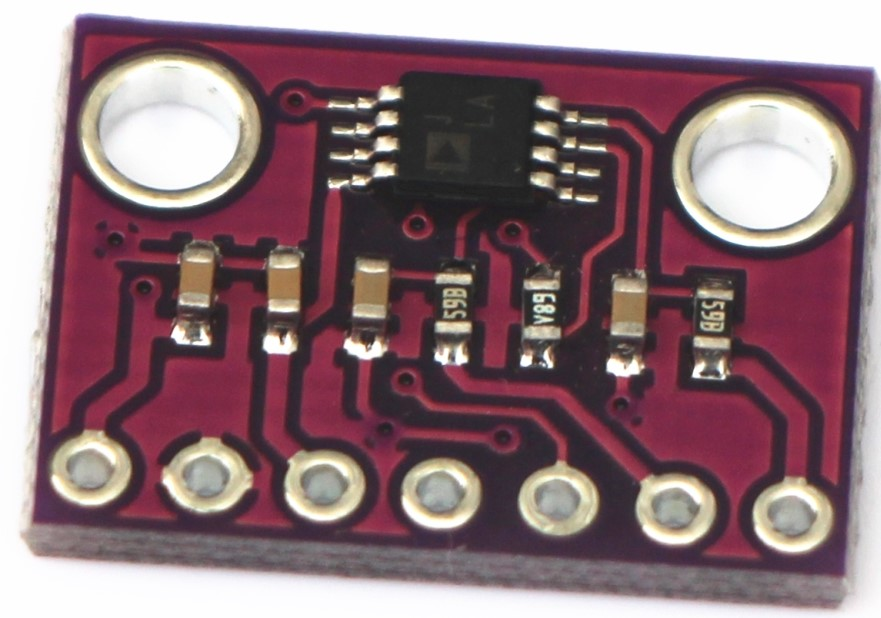
\includegraphics[width=0.4\textwidth]{../images/InstAmpBreakoutBottom.jpg}

where pin 1 is GND, pin 2 is the data line, and pin 3 is NC on old systems and 3.3v or GND on new ones (Ground for parasitic).  The data line needs a pull-up resistor\footnote{A resistor that supplies power to a bus, connected between the data and 3.3v in our case.} of around 3k$\Omega$ to 6k$\Omega$, with the sugested value at 4.7k$\Omega$. The one wire thermometer is very easy to connect to a Raspberry pi.  Connect pin 1 to ground, pin 2 to GPIO 4 (4th pin on the left of the Raspberry Pi's GPIO), and pin 3 to 3.3 volts.  Now connect a resistor around 4.7k$\Omega$ between pins 2 and 3 of the one wire.  You are ready to set up your Pi!

\section{Add One Wire Support}

First you need to edit the boot configuration file to add one wire support.

\CommandLine{sudo nano /boot/config.txt}

Scroll to the bottom (use the down arrow), then type \textbf{dtoverlay=w1-gpio}.
Save by typing \textbf{ctrl-o} then exit with \textbf{ctrl-x}.

Now reboot to make your changes active.


\CommandLine{sudo reboot}

\section{Test It}


\CommandLine{sudo modprobe w1-gpio}

\CommandLine{sudo modprobe w1-therm}



\CommandLine{cd /sys/bus/w1/devices}

\CommandLine{ls}

Note that the next directory has a really long name, and incorporates the device number so it is not constant on all systems.  This allows multiple to be connected.


\CommandLine{cd 28*}


\CommandLine{cat \url{w1_slave}}

\section{Code It}

\Code{Read from a One Wire Thermometer.}{code:w1}{../labs/lab_04/w1temp.py}{Python} 